\documentclass[border=3pt,tikz]{standalone}
\usepackage{bm,amsmath}
\usetikzlibrary{patterns,decorations.pathmorphing}
\usetikzlibrary{arrows.meta}
\usetikzlibrary{calc}

\begin{document}

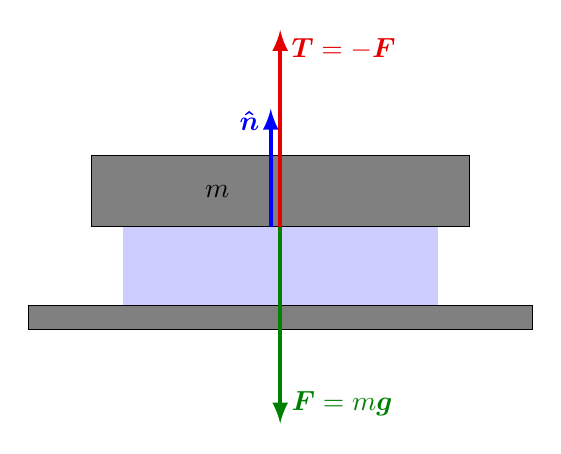
\begin{tikzpicture}
    \def\L{4}
    \def\H{1}
    \def\h{0.3}

    \coordinate (O) at (0,0);
    \fill[blue!20] (O)--++(\L,0)--++(0,\H)--++(-\L,0)--cycle;
    \draw[fill=gray] ($(O)-(0.3*\L,0)$)--++(1.6*\L,0)--++(0,-\h)--++(-1.6*\L,0)--cycle;
    \draw[fill=gray] ($(O)+(-0.1*\L,\H)$)--++(1.2*\L,0)--++(0,3*\h)--++(-1.2*\L,0)--cycle;
    \node at ($(O)+(0.3*\L,\H+1.5*\h)$) {$m$};

    \draw[-latex,ultra thick,green!50!black] ($(O)+(0.5*\L,\H)$)--++(0,-2.5*\H) node[right,pos=0.9] {$\bm{F}=m\bm{g}$};

    \draw[-latex,ultra thick,blue] ($(O)+(0.47*\L,\H)$)--++(0,1.5*\H) node[left,pos=0.9] {$\bm{\hat{n}}$};
    \draw[-latex,ultra thick,red!90!black] ($(O)+(0.5*\L,\H)$)--++(0,2.5*\H) node[right,pos=0.9] {$\bm{T}=-\bm{F}$};
\end{tikzpicture}

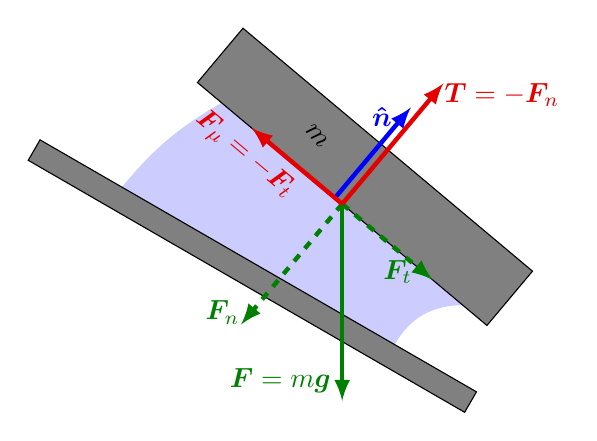
\begin{tikzpicture}
    \def\L{4}
    \def\H{1}
    \def\h{0.3} 

    \coordinate (A) at (0,0);
    \fill[blue!20] (A)--++(-30:\L) coordinate (B) to[bend left=30] ++(30:\H) coordinate (C)--++(180-40:\L) coordinate (D) to[bend right=10] cycle;

    \draw[fill=gray] ($(A)+(-30:-0.3*\L)$)--++(-30:1.6*\L)--++(-30-90:\h)--++(-30:-1.6*\L)--cycle;
    \draw[fill=gray] ($(D)+(-40:-0.1*\L)$)--++(-40:1.2*\L)--++(90-40:3*\h)--++(-40:-1.2*\L)--cycle;
    \node[rotate=-50] at ($(D)!0.3!(C)+(50:1.5*\h)$) {$m$};
    \draw[-latex,ultra thick,green!50!black] ($(D)!0.5!(C)$)--++(0,-2.5*\H) node[left,pos=0.9] {$\bm{F}=m\bm{g}$};
    \draw[-latex,ultra thick,dashed,green!50!black] ($(D)!0.5!(C)$)--++(-90-40:2*\H) node[left,pos=0.9] {$\bm{F}_n$};
    \draw[-latex,ultra thick,dashed, green!50!black] ($(D)!0.5!(C)$)--++(-40:1.5*\H) node[left,pos=0.9] {$\bm{F}_t$};
    \draw[-latex,ultra thick,blue] ($(D)!0.47!(C)$)--++(50:1.5*\H) node[left,pos=0.9] {$\bm{\hat{n}}$};
    \draw[-latex,ultra thick,red!90!black] ($(D)!0.5!(C)$)--++(50:2*\H) node[right,pos=0.9] {$\bm{T}=-\bm{F}_n$};
    \draw[-latex,ultra thick,red!90!black] ($(D)!0.5!(C)$)--++(-40:-1.5*\H) node[below,pos=0.9,rotate=-40] {$\bm{F}_\mu=-\bm{F}_t$};

\end{tikzpicture}

\end{document}